\chapter{Моделирование динамики доходности торговых стратегий}
\section{Выбор парадигмы моделирования: частотный и байесовский подходы}
\note{Зачем тут байесовский подход?}
Существует две парадигмы для моделирования -- частотный подход и байесовский. Каждая из них обладает своими преимуществами и недостатками \citep{gelman2008}:
\begin{table}[h]
\centering
\caption{Сравнение байесовской и частотной парадигмы}
	\begin{tabular}{l|c|c}
	& Байесовский  & Частотный \\ \hline
	Трактование вероятности & мера знания & частота события \\ \hline
	Параметры модели & случайные величины & неизвестные константы \\ \hline
	Данные & \multicolumn{2}{c}{из неизвестного распределения}  \\ \hline
	Учет априорных знаний & да & нет \\ \hline
	Необходимость большой выборки & нет & да
 	\end{tabular}
\end{table}

Составление портфеля торговых стратегий -- практическая задача, решаемая инвестиционным фондом. Существуют процессы создания алгоритмов вовлекающие посторонних людей, они участвуют на конкурсной основе и результатом их работы являются торговые стратегии. Конкурсная основа мероприятия смещает стимулы участников, как следствие, создаются алгоритмы хорошо работающие на бэктесте, но в реальной ситуации ведут себя непредсказуемо. Следуя байесовскому подходу это можно выразить в априорном распределении на доходности <<до>> и <<после>> создания алгоритма. Традиционный частотный подход не способен в полной мере отразить существенную разницу между этими периодами, кроме как структурно.

База стратегий огромная, для применения портфельной теории необходимо выбрать подмножество и работать с ним. Этот отбор так же влияет на то, какие алгоритмы участвуют в построении портфеля, меняются и предположения о распределении доходностей торговых стратегий, их волатильности и динамике. Частотный подход не способен учесть экспертные знания о влиянии процедуры отбора на финальную выборку.

Байесовский подход является предпочтительным, он позволяет учесть экспертные знания в модели и неопределенность в параметрах как самой модели, так и ее предсказаний относительно будущей динамики.
\section{Учет специфики динамики доходностей в рамках байесовского подхода}
\subsection{Моделирование сдвигов доходностей}
\note{Модель структурных сдвигов}
Для учета структурных сдвигов с известной точкой перехода можно использовать две различные модели <<до>> и <<после>> \citep{salazar1982}. Этот подход -- естественная идея, кроме того, есть свобода учитывать структурные изменения лишь в тех частях модели, которые в этом нуждаются, как например средние доходности.

\subsection{Моделирование волатильности доходностей во времени}
\note{Обзор методов моделирования волатильности}
Для учета стохастической волатильности используется класс моделей имеющих скрытый марковский процесс \citep{ghahramani2001}:
\begin{itemize}
	\item GARCH \citep{engle1982}
	\item Gaussian Process Volatility Model (GPVol) \citep{han2016}
\end{itemize}
Семейство GPVol гораздо богаче чем GARCH -- оно непараметрическое. К тому же модель GPVol относительно проста в реализации и встраивается в байесовский подход.

\note{про гауссовский процесс, много, для воды}
\paragraph{Гауссовский процесс} -- непараметрическое априорное распределение над функциями. Оно широко используется при байесовском моделировании и позволяет оценить неизвестную функцию. В контексте задачи моделирования временных рядов, такой функцией будет скалярная функция от времени, описывающая динамику временного ряда.
\begin{figure}[h]
	\centering
	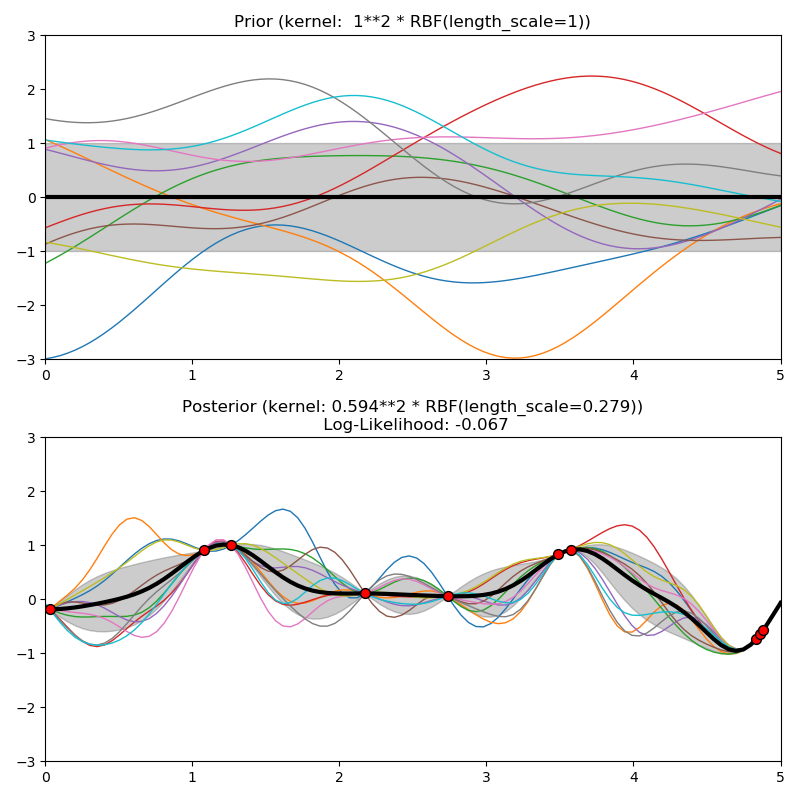
\includegraphics[width=0.7\linewidth]{sampleGP}
	\caption{Пример Гауссовского Процесса}
\end{figure}
Важным достоинством гауссовского процесса над другими моделями временных рядов являются его интерпретируемость, легкость имплементации и оценки. Что важно для приложения к задаче построения модели и учета априорных знаний, это интерпретируемость параметров. В ней главными являются значения среднего и магнитуды. В них можно учесть предположения о безусловном распределении доходностей алгоритмов.
\begin{align}
	f \sim \mathcal{GP}(m, k) \iff \E{f(x)} = m(x),\quad \E{(f(x) - m(x))(f(x')-m(x'))} = k(x, x'),
\end{align}
Где $m$ -- функция от $x$, но так же может быть и константой. Если считать, что доходности распределены по гаусовскому процессу, то параметр среднего можно интерпретировать, как среднюю доходность, магнитуду как средний риск. В работе будет рассмотрен гауссовский процесс с гауссовским ядром $k(x, x')=exp(-\tfrac{||x-x'||^2}{2\sigma^2})$.

Но в постановке GPVol, волатильность -- непостоянный параметр, этого можно добиться дополнительно введя шум на доходности, дисперсия которого подчиняется гауссовскому процессу.

\begin{align}
	r_m(t) & \sim GP_m\\
	r_v(t) & \sim GP_v\\
	r(t) & = r_m(t) + t_v(t)
\end{align}

\note{учет сдвига в моделях волатильности}
Волатильность -- косвенный показатель, и он не учитывается автором в явном виде. Поэтому процесс стохастической волатильности будем считать неизменным до и после структурного сдвига. Тем временем параметры среднего для процесса на средние доходности будут различаться <<до>> и <<после>> структурного сдвига.

\subsection{Моделирование динамики корреляций доходностей во времени}
\note{в чем сложность моделирования динамики корреляций?}
Моделирование динамики корреляций -- сложная задача, это скрытый марковский процесс с большим количеством скрытых состояний, квадратичным по количеству рядов. Без априорных предположений о структуре матрицы корреляций, вычислительная сложность слишком велика. Существует несколько основных подходов для моделирование динамики корреляций.
\begin{itemize}
	\item Dynamic Conditional Correlation (DCC) \citep{engle2000}
	\item Dynamic Equicorrelation Stochastic Volatility (DECO) \citep{kurose2016}
\end{itemize}
DCC модель моделирует динамику всей ковариационной матрицы, но не работает уже при хоть сколько нибудь значимой размерности. DECO модель берет свои истоки из DCC с дополнительной предпосылкой: существуют группы временных рядов, для которых парные корреляции одинаковы. Это позволяет снизить вычислительную сложность и уменьшить количество оцениваемых параметров.
\begin{align}
u_t &= \frac{\sum_{i\neq j} r_i r_j}{(n-1) \sum_{i} r_i^2}\\
\rho_{t+1} &= w + \alpha u_t + \beta \rho_t, \quad w/(1-\alpha-\beta) \in \left(\tfrac{-1}{n-1}, 1\right)
\end{align}
\note{что из этого можно использовать}
Сложность задания параметрической модели состоит в недостаточно подробном руководстве авторов статьи к имплементации. Более того, рекуррентные соотношения в вычислительном графе будут негативно сказываться на скорость вычислений. 
Естественным продолжением этой модели является гауссовский процесс для $\rho_t$ используя соответствующее  биективное преобразование $T:\: \mathbb{R} \to \left(\tfrac{-1}{n-1}, 1\right)$. Из-за гибкости и удобства моделирования этот метод и будет использован в итоговой спецификации.
На основании вышеизложенных причин, было решено использовать модификацию с гауссовским процессом, который не страдает от изложенных недостатков.

\begin{equation}
	\kappa_t = logit((\rho_t + \tfrac{1}{n-1} )/\tfrac{n}{n-1}))  \sim \mathcal{GP},
\end{equation}
где статистика $\kappa_t \in \Real$ и распределена согласно гауссовскому процессу. Такая параметризация крайне удобна, так как лишает необходимости задавать параметрический процесс. 

\section{Формирование модели динамики доходностей торговых стратегий: анализ различных спецификаций}
Объединяя части в одно целое, получим генеративную модель, учитывающую динамику корреляций торговых стратегий:
\paragraph{Расширенная спецификация с динамикой корреляций (DynCorr)}

\begin{align*}
\mu_\text{is} &\sim p(\mu_\text{is}); \in \Real^k& \text{ожидаемая доходность в обучающем периоде}\\
\mu_\text{oos} &\sim p(\mu_\text{oos});\in \Real^k&\text{ожидаемая доходность в тестовом периоде}\\
\nu &\sim p(\nu);\in \Real^k&\text{ожидаемый логарифм дисперсии}\\
\kappa &\sim p(\kappa);\in \Real& \text{ожидаемая статистика корреляции}\\
\theta_\mathcal{GP} &\sim p(\theta_\mathcal{GP})&\text{параметры многомерного гауссовского процесса}\\
\phi_\mathcal{GP} &\sim p(\phi_\mathcal{GP})&\\
\psi_\mathcal{GP} &\sim p(\psi_\mathcal{GP})&\\
\Delta\mu &\sim \mathcal{GP}(\theta_\mathcal{GP}); f:\Real \to \Real^k&\text{изменение доходности во времени}\\
\Delta\nu &\sim \mathcal{GP}(\phi_\mathcal{GP}); f:\Real \to \Real^k&\text{изменение логарифма дисперсии во времени}\\
\Delta\kappa &\sim \mathcal{GP}(\psi_\mathcal{GP}); f:\Real \to \Real&\text{изменение статистики корреляции во времени}\\
\end{align*}
\begin{align}
\mu_t &= \begin{cases}
\mu_\text{is} + \Delta\mu(t), t \in \text{\{обучающий период\}}\\
\mu_\text{oos} + \Delta\mu(t), t \in \text{\{тестовый период\}}
\end{cases}&\text{среднее доходностей в момент t}\nonumber\\
\sigma^2_t &= \exp(\nu + \Delta\nu(t))& \text{дисперсия доходностей в момент t}\nonumber\\
\rho_t &= \tfrac{k}{k-1}(\text{sigmoid}(\kappa + \Delta\kappa(t))-\tfrac{1}{k-1})&\text{корреляция доходностей в момент t}\nonumber\\
\Sigma_t &= ((1-\rho_t)\mathbb{I} + \rho_t) \odot \sigma_t\sigma_t^\top&\text{ковариационная матрица в момент t}\nonumber\\
R_t &\sim \mathcal{N}(\mu_t,\Sigma_t)& \text{наблюдаемые доходности в момент t}\label{eq:dyncorr}
\end{align}
где $k$ -- количество алгоритмов. Априорные распределения задаются исходя из природы данных и не могут быть указаны на этом этапе.

Априорные распределения играют важную роль в моделировании, их подбор субъективная задача. Она выполняется совместно с экспертами в области. В частности, большую поддержку оказали в Quantopian при проведении экспериментальной части. Благодаря экспертным знаниям получается учесть не только структурную составляющую зависимостей в модели, но также и априорные знания о параметрах. Это позволяет на малом наборе данных получать качественную модель, игнорировать выбросы, избегать эффекта переобучения. Так, априорное распределение на ожидаемые доходности формируется с учетом этапа селекции, который, как ожидается, отбирает наиболее стабильные алгоритмы из общей массы.

Обычной практикой является введение гипераприорного распределения -- арпиорное распределение на параметры априорного распределения. Оно позволяет сгладить возможно неудачный выбор фиксированных параметров априорного распределения и выражает неуверенность в изначальных предположениях. Эти подходы хорошо описаны например в \cite{daniel2014}. В этой работе гиперприоры -- широко используются еще и для моделирования некоторых других параметров, например стандартного отклонения для априорного распределения на средние доходности. Для упрощения выкладок гипераприорные распределения опущены в выкладках.

Несмотря на гибкость байесовского подхода остается проблематичным учесть неопределенность в структуре самой модели. Введение компоненты нестабильности корреляций во времени существенно усложняет модель как структурно, так и вычислительно. Гипотеза о необходимости динамики корреляций была сформирована на основании работ по рыночным активам \citep{vaga1990, oral2017}, подтверждается ли такое наблюдение на данных о доходностях алгоритмических стратегий -- вопрос, который подлежит изучению.

\note{Как тут использовать гауссовский процесс, как подбирать ядро}
Гауссовский процесс является центральной частью модели. Этот непараметрический метод, тем не менее, требует подбора ядра для каждой отдельной задачи. Временные ряды -- особый вид данных, часто требуется учитывать сезонность или тренд \citep{taylor2017}. Одним из бизнес процессов в компании является предварительный отбор алгоритмов, его проходят около 0.05\%. Успешно отобранные алгоритмы, что самое главное, имеют стационарное распределение доходностей. Таким образом, основной предпосылкой о структуре временного ряда будет его стационарность. Гауссовское ядро выражает вводимые предпосылки функционально, поэтому я буду использовать его в своей работе, более того, оно позволяет оптимизировать некоторые вычисления. 

Возможны альтернативные спецификации модели, которые учитывают не динамику корреляций, а наоборот, статику.
\note{переделать не списком, разжевать каждую спецификацию}
\paragraph{Спецификация со статическими корреляциями (Corr).}
Расширенная спецификация допускает упрощения. В случае, если не будет выявлено динамической корреляции в данных, осмысленно использовать спецификацию, которая вводит дополнительную предпосылку о неизменности корреляций. Более жесткие предпосылки не делают модель беднее. Напротив, предыдущая спецификация не позволяла иметь корреляции между подгруппами алгоритмов, и ковариационная матрица имеет блок диагональный вид. Эта же, напротив, позволяет оценивать полную ковариационную матрицу, хоть и постоянную во времени.
\begin{align}
L &\sim p(L);\in R^{k\times k}:\; L_{ii} > 0 & \text{нижняя треугольная матрица}\nonumber\\
\tilde{\Sigma} &= LL^\top & \text{<<средняя>> ковариационная матрица}\nonumber\\
\Sigma_t &= \tilde{\Sigma} \odot \sigma_t\sigma_t^\top & \text{ковариационная матрица в момент t}\label{eq:staticcorr}
\end{align}

Стоит отметить, что априорное распределение задается сразу в виде $p(\tilde{\Sigma})$, причем возможно одновременно контролировать как корреляции, так и дисперсии. Основным инструментом здесь является LKJ распределение \citep{lewandowski2009} на параметры корреляций. Оно позволяет контролировать число скоррелированных компонент: от диагональной ковариационной матрицы до плотной, где корреляций много. Это распределение рекомендовано использовать вместо Inverse Wishart \citep{haff1979}, которое не обладает хорошими свойствами интерпретируемости. 

Априорное распределение на дисперсии задается отдельно, как правило оно логнормальное, что и было использовано в данной работе. Альтернативой являются распределения с тяжелыми хвостами, как Half Cauchy или Half StudentT \citep{gelman2006scale}. 

\paragraph{Спецификация без корреляций (Diag).}
Принцип <<Бритвы Оккама>> -- лучше та модель, что максимально просто объясняет природу данных. Следуя этому принципы вводится в рассмотрение дополнительная спецификация, которая вообще исключает корреляции. Она более устойчива, проста в оценке. Не исключено, что более простая модель хорошо подойдет для практических задач.

\begin{equation}
\Sigma_t = diag(\sigma^2_t)\label{eq:nocorr}
\end{equation}

\note{Часть о достоинствах и недостатках спецификаций}
У каждой спецификации есть свои достоинства и недостатки. Так, даже расширенная спецификация \eqref{eq:dyncorr} в некоторых случаях может уступать более простой модели без динамики корреляций \eqref{eq:staticcorr}. Связано это с тем, что моделировать динамику полной ковариационной матрицы чрезвычайно трудная задача и приходится вводить предпосылку о структуре ковариационной матрицы. 

Вычислительные ресурсы, требуемые на оценку модели так же различаются. Модель \eqref{eq:staticcorr} слабо масштабируется по числу алгоритмов $k$, для которых производится оценка динамики, из-за требуемых объемов памяти: $\mathcal{O}(k^2)$ для хранения ковариационной матрицы. Модель учитывающая динамику корреляций избегает этой проблемы, однако требует большого количества вычислительных ресурсов.
\begin{table}[h]
	\caption{Сравнение спецификаций модели динамики доходностей финансовых стратегий по ключевым показателям}
	\begin{tabular}{l|c|c|c}
		& DynCorr \eqref{eq:dyncorr} & Corr \eqref{eq:staticcorr}& Diag \eqref{eq:nocorr} \\ \hline
		Динамика корреляций & $+$ & $-$ & $-$ \\ \hline
		Полная ковариационная матрица &$-$ & $+$ & $-$ \\ \hline
		Динамика волатильности  &$+$ & $+$ & $+$ \\ \hline
		Сложность оценки, ч. работы сервера &10 & 3 & $<1$ \\ \hline
		Масштабируемость по числу алгоритмов & Низкая & Средняя & Высокая
	\end{tabular}
\end{table}

Необходимая спецификация будет определяться исходя из предварительного эмпирического анализа. Итоговая модель, ее апостериорное распределение, будет оцениваться с помощью Markov Chain Monte Carlo метода NUTS \citep{hoffman2011nuts} семейства Hamiltonian Monte Carlo с имплементацией на языке \texttt{Python} в пакете PyMC3 \citep{salvatier2016pymc3}\footnote{К сожалению, из-за соглашения NDA, код проекта не публикуется}.

\paragraph{Hamiltonian Monte Carlo (HMC)} -- семейство методов, использующая информацию второго порядка (градиенты) для построения марковской цепи. Основной принцип заключается в использовании гимильтоновой динамики (понятие пришло из физики) чтобы получать симуляции из распределения, не имеющего нормализующей константы в явном виде. Обычно такая сложность возникает ввиду невозможности численного интегрирования по многим переменным.
\begin{equation}
p(x) \propto exp(-\tfrac{U(x)}{T})
\end{equation}
Модель представлена системой от позиции и скорости. Вместе они формируют энергию потенциальную и кинетическую:

\begin{equation}
E(x, v) = U(x) + K(v),\quad K(v)\sum_{i}\tfrac{mv^2}{2}
\end{equation}
Совместное же распределение $p(x, v)$ раскладывается на два независимых

\begin{equation}
p(x, v) \propto exp(-\tfrac{E(x, v)}{T}) = exp(-\tfrac{U(x)}{T})exp(-\tfrac{K(v)}{T})=p(x)p(v)
\end{equation}
Используя гамильтонову динамику мы можем сэмплировать из $p(x)$. Для этого необходимо сэмплировать $v \sim p(v)$, а далее, используя тождества из физики, преобразовать $x$ по следующей динамике:
\begin{equation}
\dot{x} = v,\quad m\dot{v} = \frac{\partial U(x)}{\partial x} \label{eq:hmctraj}
\end{equation}
Однако, используя исключительно динамику, так не получится по-настоящему сэмплировать из-за закона сохранения энергии. Поэтому траектории ограничены и скорость обновляется перед каждой симуляцией динамики. Но и тут не все гладко, необходимо проводить траектории \eqref{eq:hmctraj}, обычно используют leapfrog метод для этого.

\paragraph{No U-Turn Sampler (NUTS)} -- модификация обычного HMC, с поиском оптимальной длины интегрирования \eqref{eq:hmctraj}. На сегодняшний день он остается надежным методом, способным решать среднего размера задачи байесовского вывода. Существуют уже готовые реализации этого метода и ими удобно пользоваться \citep{salvatier2016pymc3}.

\paragraph{Альтернативные методы вывода}, например вариационные методы \citep{alp2015, jimenez2015, louizos2017}, вряд ли будут адекватно подходить под эту задачу, их основное преимущество состоит в том, что они работают в условиях большой размерности параметров и больших данных; это не наш случай. У нас данных мало и количество параметров не огромно. Более того, вариационные методы не всегда хорошо улавливают связи в распределении, что зачастую приводит к нежелательным последствиям. В работе не используются вариационные методы, поскольку основная рекомендация использовать HMC, пока он работает, иначе -- вариационные методы.
\section{Составление портфеля торговых стратегий на основе модели динамики доходностей}
Вероятностная модель задает распределение над возможными траекториями доходностей группы алгоритмов. С помощью байесовского вывода возможно оценить распределение на параметры, по реальным данным $p(\Theta\cond r_{1:T})$, после чего можно производить симуляции будущих траекторий 
\[r_{T+1:T'} \sim p(r_{T+1:T'}\cond r_{1:T}) = \int p(r_{T+1:T'}\cond\Theta, r_{1:T})p(\Theta\cond r_{1:T}) d\Theta\] 
Это позволяет учесть неопределенность реального поведения доходностей в будущем для формирования портфеля из торговых стратегий.

Используя выпуклую оптимизацию будем составлять портфель, который максимизирует изоэластичную функцию полезности:

\begin{minipage}{0.4\linewidth}
\begin{equation}
U_\rho(r) = \begin{cases}
\frac{r^{1-\rho}-1}{1-\rho}, &\rho\ne 1\\
\ln r, &\rho = 1
\end{cases}
\label{eq:isoelastic}
\end{equation}
\end{minipage}
\begin{minipage}{0.5\linewidth}
	\begin{figure}[H]
		\centering
		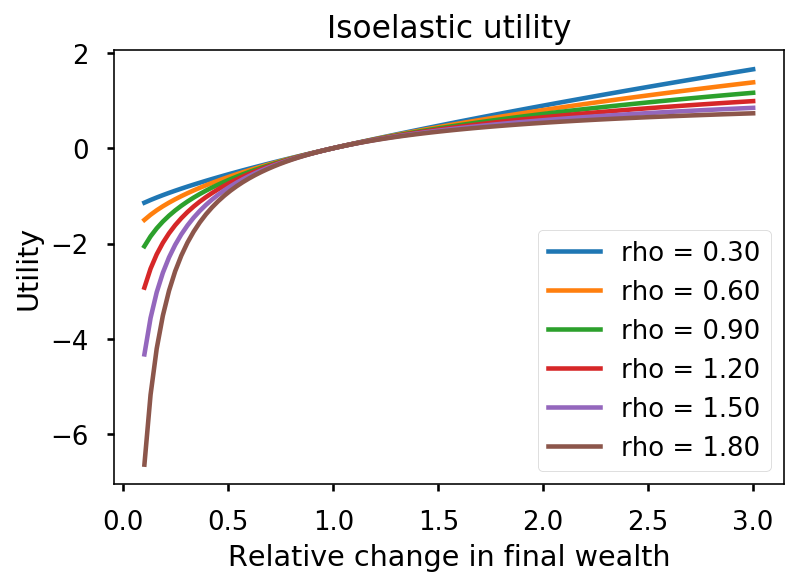
\includegraphics[width=0.7\linewidth]{Thesis/images/isoelastic}
		\caption{Изоэластичная функция полезности, При $\rho=0$ она риск нейтральна, при $\rho \to \infty$ достигается абсолютное избегание риска.}
		\label{fig:isoelastic}	
	\end{figure}
\end{minipage}
\vspace{.5cm}

 Для составления портфеля максимизируется  матожидание полезности. Выбранная функция обладает свойством избегания риска: потери учитываются в большей степени, чем выигрыши. Оптимальный портфель будет учитывать эти предпочтения.
\begin{align}
&r_{T+1:T'} \sim p(r_{T+1:T'}\cond r_{1:T})\\
&r^w = -1 + \prod_{t=T+1}^{T'} w^\top(r_t + 1)\\
&\Eb[r^w]{U_\rho(r^w)} \to \max_w, \quad w>0,\quad \sum w = 1
\end{align}
